%!TEX root = skripsi.tex
%-----------------------------------------------------------------------------%
\chapter{\babDua}
%-----------------------------------------------------------------------------%
Bab ini membahas mengenai studi literatur yang digunakan selama penelitian. Studi literatur ini menjelaskan tentang hal-hal mendasar yang dibutuhkan dalam penelitian.

%-----------------------------------------------------------------------------%
\section{Textual Entailment}
%-----------------------------------------------------------------------------%
\textit{Textual Entailment} adalah penelitian di bidang NLP yang bertujuan untuk mengidentifikasikan apakah terdapat hubungan \textit{entailment} di antara dua buah teks \citep{dagan2005}. Sebuah teks yang disebut sebagai T dikatakan meng-\textit{entail} teks lain yang disebut hipotesis atau H apabila makna teks H menjadi benar jika T diketahui benar. Hubungan \textit{textual entailment} menggambarkan bahwa dalam suatu bahasa ada beragam cara untuk menyatakan sebuah makna ke dalam bentuk teks.

\textit{Textual entailment} memiliki keterkaitan yang erat dengan fenomena parafrase. Parafrase adalah bentuk dari \textit{textual entailment} dua arah, yaitu T \textit{entail} H dan sebaliknya H \textit{entail} T. Sebagai contoh, diberikan teks berikut:

(K1): Ibu pergi ke pasar ditemani oleh ayah.

(K2): Ayah dan ibu pergi bersama.

(K3): Ayah dan ibu pergi bersama ke pasar.

(K4): Ayah tidak menemani ibu ke pasar.

(K5): Ayah membawa motor.

\noindent K1 dan K2 memiliki hubungan \textit{textual entailment} ketika K1 diposisikan sebagai T dan K2 sebagai H. Sedangkan, hubungan antara K1 dan K3 adalah parafrase karena K1 \textit{entail} K3 dan sebaliknya K3 \textit{entail} K1. Di sisi lain, K1 tidak \textit{entail} K4 maupun K5 karena makna kedua kalimat tidak dapat diperoleh dari informasi yang diberikan K1.

Pada beberapa penelitian \textit{Textual Entailment}, salah satunya yang dilakukan oleh \cite{giampiccolo2008fourth}, hubungan T tidak \textit{entail} H dibagi menjadi dua jenis, yaitu \textit{contradiction} dan \textit{unknown}. \textit{Contradiction} terjadi apabila makna T dan H saling berlawanan, yaitu T benar maka H menjadi salah dan sebaliknya. \textit{Contradiction} tergambar dari hubungan K1 dengan K4 atau K3 dengan K4. Sedangkan, hubungan \textit{unknown} terjadi apabila kebenaran H tidak dapat ditentukan oleh T, seperti saat K1 menjadi T dan K5 menjadi H.

Menurut \cite{Androutsopoulos:2010:SPT:1892211.1892215} ada tiga sudut pandang pekerjaan dalam \textit{Textual Entailment}, yaitu \textit{Textual Entailment Recognition}, \textit{Textual Entailment Extraction}, \textit{Textual Entailment Generation}. \textit{Textual Entailment Recognition} bertujuan untuk mengindentifikasi apakah ada hubungan \textit{entailment} antara sepasang teks, salah satu cara menyelesaikan masalah tersebut adalah dengan klasifikasi. \textit{Textual Entailment Extraction} adalah penelitian yang bertujuan untuk menemukan atau mengekstrak pasangan teks yang berpotensi memiliki hubungan \textit{entailment}. Sedangkan, dalam \textit{Textual Entailment Generation} hubungan \textit{entailment} tidak diidentifikasi melainkan dibangun, misalnya dengan menggunakan \textit{template} berupa pasangan-pasangan teks yang memiliki hubungan \textit{entailment}.

	\subsection{Tingkatan Textual Entailment}
	Fenomena \textit{textual entailment} dapat terjadi dalam beberapa kategori tingkatan. \cite{BENTIVOGLI10.478} di dalam penelitiannya menyimpulkan terdapat lima tingkatan \textit{Textual Entailment}, yaitu leksikal, sintaktik, leksikal-sintaktik, \textit{discourse} dan \textit{reasoning}. 
		
	Pada tingkatan leksikal, perbedaan T dan H umumnya hanya berupa perubahan kata tertentu saja, seperti menggantikan sebuah kata dengan sinonim kata tersebut atau mensubstitusi suatu istilah dengan akronimnya. Pada tingkatan sintaktik, T dan H mengalami perubahan struktur tata bahasa. Sedangkan, Hubungan T dan H pada tingkatan leksikal-sintaktik digambarkan melalui perbedaan leksikal maupun tata bahasa teks tersebut. Tingkatan \textit{discourse} mencakup hubungan yang lebih luas daripada sebuah kalimat. Hubungan T dan H pada tingkatan \textit{discourse} dipertimbangkan juga berdasarkan teks yang berada sebelum atau sesudah teks tersebut. Pada tingkatan \textit{reasoning}, dibutuhkan informasi atau pengetahuan lain agar dapat mengidentifikasikan hubungan antara T dan H.
	
	Tabel \ref{table:tingkat-TE} menunjukkan contoh pada masing-masing tingkatan. Variasi fenomena tidak mutlak berada pada tingkatan yang tertera pada tabel. Beberapa fenomena juga tidak ditemui pada Bahasa Indonesia.
	\begin{table}
		\centering
		\caption{Tingkatan Textual Entailment}
		\label{table:tingkat-TE}
		\begin{tabular}{|p{2cm}|p{4cm}|p{7cm}|}
			\hline
			Tingkatan & Variasi Fenomena & \multicolumn{1}{l|}{Contoh} \\ \hline 
			\multirow{6}{*}{leksikal} & \multirow{6}{4cm}{identitas, format, akronim, demonim, sinonim, oposisi semantik, hipernim, pengetahuan geografis} & Akronim \\
			&  & T: Fasilkom berada di dekat perpustakaan UI \\
			&  & H: Fakultas Ilmu Komputer berada di dekat perpustakaan UI \\
			&  & Sinonim \\
			&  & T: Masakan buatan ibu sangat lezat \\
			&  & H: Masakan buatan ibu sangat sedap \\ \hline
			\multirow{3}{*}{sintaktik} & \multirow{3}{4cm}{\textit{transparent heads}, nominalisasi/verbalisasi, kausatif, parafrase} & Kausatif \\
			&  & T: Para pekerja melebarkan jalan \\
			&  & H: Para pekerja membuat jalan menjadi lebar \\ \hline
			\multirow{6}{2cm}{leksikal-sintaktik} & \multirow{6}{4cm}{negasi, \textit{modifier}, realisasi argumen, aposisi, \textit{list}, kordinasi, aktif-pasif, \textit{alternation}.} & Aktif-pasif \\
			&  & T: Kue tersebut dimakan adik \\
			&  & H: Adik memakan kue itu \\
			&  & Aposisi: \\
			&  & T: Barack Obama menyukai nasi goreng \\
			&  & H: Presiden kulit hitam pertama AS menyukai nasi goreng \\ \hline
			\multirow{3}{*}{\textit{discourse}} & \multirow{3}{4cm}{\textit{coreference}, aposisi, \textit{zero anaphora}, \textit{ellipsis}, \textit{statement}.} & \textit{Coreference} \\
			&  & T: Adik menghabiskan kue tersebut karena adik menyukai kue itu \\
			&  & H: Adik menghabiskan kue tersebut karena adik menyukainya \\ \hline
			\multirow{9}{*}{\textit{reasoning}} & \multirow{9}{4cm}{oposisi, \textit{modifiers}, \textit{genitive}, klausa relatif, \textit{elliptic expressions}, meronim, metonimia, \textit{reasoning on quantities}, semua penurunan kalimat menggunakan pengetahuan dasar.} & Oposisi: \\
			&  & T: Sebagian orang menggunakan bus \\
			&  & H: Sebagian orang tidak menggunakan bus \\
			&  & \textit{Elliptic expression}: \\
			&  & T: Ayah makan bakso.  Ibu makan bakso. \\
			&  & H: Ayah makan bakso, begitu juga ibu. \\
			&  & Metonimia: \\
			&  & T: Ayah membeli Djarum Coklat \\
			&  & H: Ayah membeli rokok \\ \hline
		\end{tabular}
	\end{table}
	
	\subsection{Pemanfaatan Textual Entailment}
	Keragaman dalam menyatakan suatu makna ke dalam teks adalah fenomena yang lumrah terjadi di bidang \textit{Natural Language Processing} (NLP), seperti dalam pengembangan sistem \textit{Question Answering} (QA), \textit{Information Extraction} (IE), \textit{Information Retrieval} (IR), \textit{Machine Translation}, dan \textit{Summarization} \citep{dagan2004}. Ide dari pemanfaatan fenomena \textit{textual entailment} dan parafrase dalam penelitian NLP bahkan muncul sebelum penelitian \textit{Textual Entailment} dikembangkan, seperti yang dilakukan \cite{shinyama2003paraphrase} untuk IE \textit{system} dan \cite{Radev:2000:CTI:1117736.1117745} untuk sistem \textit{Summarization}. 
	
	\textit{Framework} aplikasi \textit{Textual Entailment} dalam penelitian QA yang umum digunakan adalah merepresentasikan pertanyaan sebagai T dan sejumlah teks calon jawaban direpresentasikan sebagai H \citep{sacaleanu-EtAl:2008:DEMOS}. Jawaban yang akan diberikan oleh sistem tersebut adalah teks pada calon jawaban yang di-\textit{entail} oleh pertanyaan. Pada salah satu penelitian QA yang dilakukan oleh \cite{harabagiu-hickl:2006:COLACL}, beberapa variasi dari \textit{QA system} menggunakan \textit{Textual Entailment} dibandingkan dengan \textit{QA system} biasa. Hasil penelitian menunjukkan semua variasi \textit{QA system} menggunakan \textit{Textual Entailment} lebih baik dibandingkan \textit{QA system} biasa.
	
	Salah satu pekerjaan dalam \textit{Information Extraction} adalah melakukan \textit{pattern matching} \citep{grishman1997information}. Potongan-potongan informasi dimasukkan ke dalam \textit{pattern} yang sudah ditentukan. Oleh karena itu, performa IE \textit{system} dipengaruhi oleh desain dari \textit{pattern} tersebut. \cite{shinyama2003paraphrase} menggunakan metode parafrase untuk memperbanyak variasi \textit{pattern} yang mengekspresikan makna yang sama. Dengan metode parafrase, kelompok \textit{pattern} yang sama bisa diperoleh dengan mudah. 
	
	Pada penelitian \textit{Summarization}, aplikasi \textit{Textual Entailment} bahkan dapat bervariasi. Salah satu penelitian mencoba memanfaatkan \textit{Textual Entailment} untuk mengevaluasi hasil rangkuman dari sistem \textit{Summarization} \citep{bhaskar-pakray:2013:RANLPStud-2013}. Sedangkan, dalam  \textit{Summarization} untuk multi-dokumen, pemanfaatan \textit{Textual Entailment} adalah untuk pendeteksian kemunculan teks yang memiliki makna serupa \citep{Radev:2000:CTI:1117736.1117745}. Teks-teks yang \textit{redundant} akan dihilangkan sehingga rangkuman menjadi lebih ringkas.

%-----------------------------------------------------------------------------%
\section{Korpus}
%-----------------------------------------------------------------------------%	
%-----------------------------------------------------------------------------%	
Korpus adalah sebuah kumpulan teks dengan format standar yang dapat dibaca oleh mesin elektronis dan dibuat berdasarkan kriteria dan tujuan yang tertentu \citep{ATKINS01011992}. Berikut adalah penjelasan mengenai kriteria dan tahap pembuatan korpus, serta contoh pembuatan korpus pada penelitian \textit{Textual Entailment}.
	
	\subsection{Kriteria dan Tahap Pembuatan Korpus}
	Secara umum, sebuah korpus yang baik adalah korpus yang berisikan data representatif \citep{xiao2010corpus}. Menurut \cite{biber1993representativeness}, definisi representatif merujuk pada kemampuan korpus dalam mencakup seluruh variasi fenomena tertentu ke dalam beberapa sampel. Representatif diperoleh apabila data yang tersimpan di korpus merupakan \textit{sampling} dari fenomena di kondisi nyata dan setiap variasi fenomena berjumlah seimbang.
	
	Secara garis besar, ada beberapa tahap dalam pembuatan korpus \citep{ATKINS01011992}, yaitu: spesifikasi dan desain korpus, pemilihan sumber data korpus, perolehan perizinan data korpus, \textit{data capture}, dan pemrosesan korpus. Pada tahap spesifikasi dan desain, dilakukan penentuan terhadap tujuan, jenis, ukuran, dan atribut lain terkait korpus yang akan dibuat. Kemudian sumber data untuk pembuatan korpus ditentukan dan diperoleh izin penggunaannya. Pada tahap \textit{data capture}, data dari sumber diolah agar dapat berubah menjadi bentuk yang diterima oleh komputer, seperti \textit{scanning} pada kumpulan kertas dokumen atau pembuatan transkrip pada data audio. Proses terakhir adalah pemrosesan data hingga data menjadi bentuk korpus yang diharapkan. 
	
	\subsection{Korpus Textual Entailment} 
	\cite{burgerfero} pernah melakukan pengembangan secara otomatis sebuah korpus \textit{Textual Entailment} bahasa Inggris. Namun, korpus tersebut hanya berisikan data \textit{entailment} yang positif, yaitu T \textit{entail} H. Ide pembuatan korpus tersebut menggunakan \textit{headline} dari sebuah berita dan paragraf pertama berita tersebut sebagai pasangan T dan H dengan asumsi \textit{headline} dan paragraf pertama kemungkinan memiliki hubungan parafrase. Selanjutnya, \cite{dagan2005} mengembangkan korpus \textit{Textual Entailment} bahasa Inggris secara manual dengan bantuan beberapa anotator. Korpus tersebut berisikan daftar pasangan T dan H yang diberi label secara \textit{binary} yaitu \textit{true} dan \textit{false}, \textit{true} jika T \textit{entail} H dan \textit{false} jika T tidak \textit{entail} H. Kemunculan korpus-korpus tersebut mendorong banyak pihak untuk melakukan penelitian \textit{Textual Entailment}.
	
	Perkembangan \textit{Textual Entailment} bahasa Inggris terus berlanjut hingga sekarang. \cite{snli:emnlp2015} merilis korpus Stanford Natural Language Inference (SNLI), yaitu sebuah \textit{Textual Entailment} korpus berisikan 570 ribu data dengan tiga label yaitu \textit{entailment}, kontradiksi, dan netral. Ukuran korpus tersebut tergolong besar. Proses pembuatannya dilakukan manual oleh 2500 pekerja. Para pekerja diberikan sebuah teks keterangan foto tanpa diperlihatkan foto tersebut. Mereka diminta untuk membuat kalimat yang mungkin menjadi alternatif untuk menggantikan keterangan foto tersebut.
	
	Kemajuan penelitian \textit{Textual Entailment} bahasa Inggris memberi motivasi penelitian \textit{Textual Entailment} untuk bahasa lain, diantaranya Italia, Jerman, dan Spanyol. Pengembangan \textit{Textual Entailment} untuk ketiga bahasa tersebut dilakukan dengan cara yang berbeda. Pada bahasa Italia, dikembangkan korpus \textit{Textual Entailment} yang diberi nama EVALITA. EVALITA dikembangkan menggunakan data dari Wikipedia \textit{revision history} \citep{RTEevalita}. Sedangkan, pengembangan korpus \textit{Textual Entailment} Spanyol menggunakan data dari penilaian sebuah QA \textit{system} yang sudah dikembangkan sebelumnya di Spanyol \citep{RTEsparte}. Korpus \textit{Textual Entailment} Jerman dikembangkan dengan menggunakan metode \textit{crowdsourcing} \citep{RTEjerman} serupa dengan pengembangan korpus SNLI. Korpus \textit{Textual Entailment} Jepang dibuat dengan mengkombinasikan fitur-fitur \textit{entailment} dari T dan H dalam bahasa Jepang dan terjemahan dalam bahasa Inggris dari pasangan T dan H tersebut, tahap penerjemahaan disebut \textit{bilingual enrichment} \citep{pham2012empirical}. 
	
	%Selain penelitian membangun dari nol sebuah korpus \textit{Textual Entailment}, ada pula penelitian yang dialkukan untuk memperbesar ukuran korpus Textual Entailment. Penelitian tersebut dilakukan oleh \cite{zanzottoRTEexpand}.%

%-----------------------------------------------------------------------------%
\section{Wikipedia}
%-----------------------------------------------------------------------------%
Wikipedia\footnote{www.wikipedia.org} adalah ensiklopedia multi-bahasa yang dapat ditulis secara kolaboratif oleh siapa pun dari seluruh penjuru dunia \citep{wikipediaxml:2005}. Sejak kemunculan pertama Wikipedia tahun 2001, Wikipedia memperoleh pengembangan kuantitas yang sangat pesat. Situs yang dikelola oleh organisasi non profit Wikimedia Foundation ini memiliki 374 juta pengunjung unik setiap bulannya berdasarkan data pada bulan September 2015. Ada sekitar 41 juta artikel dari 294 bahasa berbeda yang ditulis oleh 70.000 kontributor aktif pada Wikipedia. Wikipedia memiliki jumlah artikel, suntingan, dan kolaborator yang sangat besar karena sifatnya yang bebas. Selain itu, proses penyuntingan artikel lebih mudah karena menggunakan Wiki \textit{markup language} yang lebih sederhana daripada bentuk HTML. 


\subsection{Wikipedia Offline}
Selain dapat diakses secara \textit{online}, Wikipedia juga tersedia dalam bentuk \textit{offline} dan dapat diunduh secara gratis melalui situs Wikimedia \textit{dumps}\footnote{https://dumps.wikimedia.org}. Wikipedia \textit{offline} tersedia dalam format XML dengan berbagai jenis, dua diantaranya adalah halaman seluruh artikel dan \textit{revision history}. Dokumen XML tersebut dimuat dalam berbagai bahasa, sesuai dengan bahasa yang digunakan Wikipedia, termasuk Bahasa Indonesia. 
\begin{figure}
	\centering
	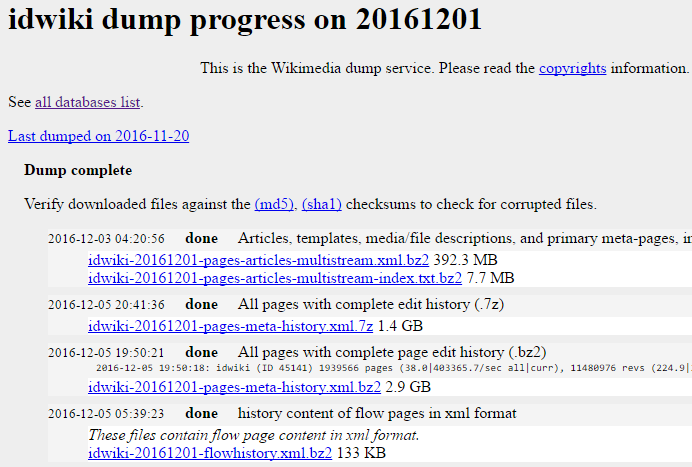
\includegraphics[width=1\linewidth]{pics/wikidumps}
	\caption{Contoh halaman Wikimedia \textit{dumps} Bahasa Indonesia}
	\label{fig:wikidumps}
\end{figure}
\noindent Pada gambar \ref{fig:wikidumps}, angka yang terdapat di judul halaman "idwiki dump progress on 20161201" menunjukkan data yang disimpan adalah data Wikipedia terakhir pada tangga 1 Desember 2016. Isi halaman tersebut adalah daftar berkas XML dari Wikipedia dengan jenis tertentu, ada pula keterangan status, tanggal pengambilan, dan ukuran berkas.		

%gambar salah satu artikel dan struktur WIkipedia

\subsection{Wiki Markup Language}
Artikel-artikel yang terdapat pada berkas XML yang tersedia di halaman Wikimedia tertulis dalam bentuk Wiki \textit{markup language} yaitu sebuah format sederhana untuk melakukan \textit{editing} pada halaman Wikipedia. Penjelasan mengenai penggunaan Wiki \textit{markup language} tersedia di salah satu halaman bantuan Wikipedia\footnote{https://en.wikipedia.org/wiki/Help:Wiki\_markup}. Format yang dapat direpresentasikan dengan Wiki \textit{markup language} antara lain, judul \textit{section}, gambar dan media lainnya (seperti animasi dan suara), tabel, daftar (\textit{list}), \textit{link}, serta format-format untuk menebalkan atau memiringkan teks. Gambar \ref{fig:wiki-xml} menunjukkan potongan artikel dalam berkas XML Wikipedia.
\begin{figure}
	\centering
	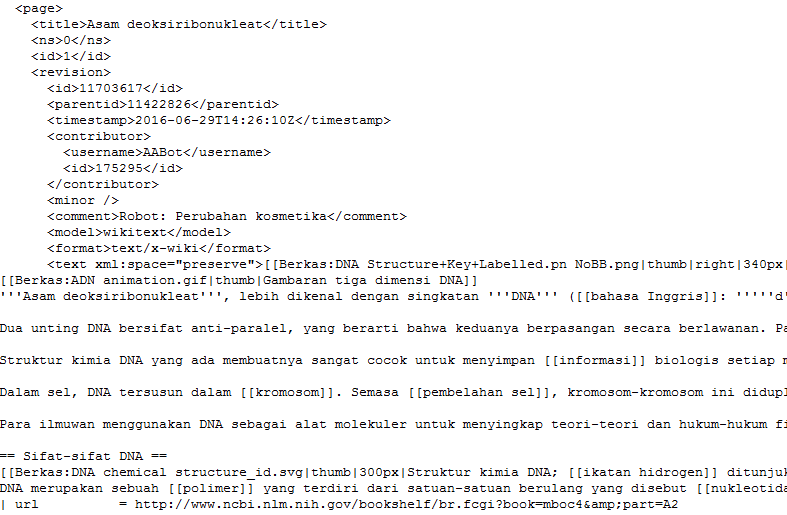
\includegraphics[width=1\linewidth]{pics/wiki-xml}
	\caption{Berkas XML artikel Wikipedia}
	\label{fig:wiki-xml}
\end{figure}
\noindent Pada gambar \ref{fig:wiki-xml}, terdapat beberapa contoh penggunaan format Wiki \textit{markup language}.
\begin{itemize}
	\item Judul \textit{section}\\
	Judul sebuah \textit{section} diapit dengan simbol sama dengan atau '=' sebanyak tingkatan \textit{section} tersebut. Contoh penggunaan judul \textit{section} pada gambar adalah penulisan "==Sifat-sifat DNA==", yang berarti "Sifat-sifat DNA" merupakan judul \textit{section} tingkat kedua.
	\item Gambar atau media\\
	Nama dari berkas gambar atau media, seperti animasi maupun suara, ditulis di dalam tanda '[[' dan ']]'. Apabila ada opsi lain untuk mengatur media tersebut, opsi diletakkan di dalam tanda kurung yang sama namun diposisikan setelah nama berkas dan dipisahkan dengan tanda '|'. Contoh penggunaan format gambar pada gambar di atas adalah "[[Berkas:ADN animation.gif|thumb|gambaran tiga dimensi DNA]]". Opsi \textit{thumb} berarti media diposisikan di kanan halaman, kemudian teks berikutnya merupakan opsi keterangan gambar.
	\item Format teks\\
	Teks yang mengalami penebalan ditandai dengan \textit{triple quote}. Sedangkan, Teks yang dimiringkan ditandai dengan \textit{double quote}.
	\item \textit{Link}\\
	\textit{Link} ditujukan untuk membuat suatu teks frasa dapat merujuk ke halaman yang terkait apabila diklik. Penulisan \textit{link} diapit oleh tanda kurung '[[' dan ']]', contoh pada gambar adalah "[[koromosom]]", "[[informasi]]", dan "[[pembelahan sel]].
\end{itemize}


\subsection{Wikipedia Revision History}
Wikipedia \textit{revision history} adalah salah satu jenis dari berkas XML yang tersedia di Wikimedia Dumps.
\begin{figure}
	\centering
	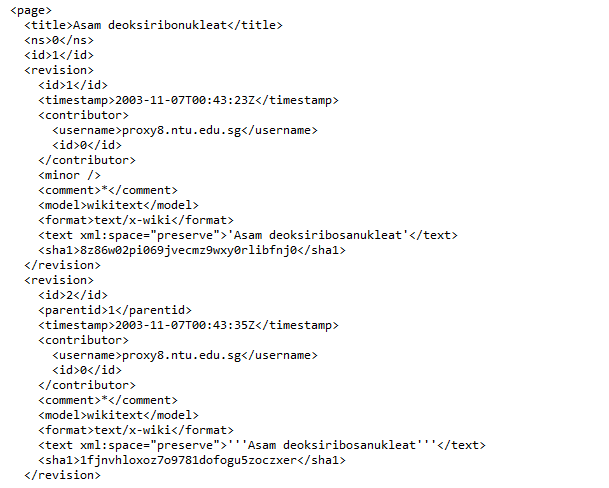
\includegraphics[width=1\linewidth]{pics/XMLWikipediaRevisionHistory}
	\caption{Berkas XML Wikipedia Revision History}
	\label{fig:wikirevisionhistory}
\end{figure}
\noindent Berkas XML Wikipedia \textit{revision history} memiliki sedikit perbedaan struktur dengan XML artikel Wikipedia umum (lihat gambar \ref{fig:wikirevisionhistory}). Sama seperti pada XML Wikipedia umum, halaman artikel ditandai dengan \textit{tag} \textit{page}. Sedangkan untuk revisi, berkas XML Wikipedia \textit{revision history} tidak hanya menyimpan revisi terakhir saja, melainkan kondisi awal artikel hingga revisi terakhir. Revisi-revisi tersebut ditandai oleh \textit{tag} \textit{revision}. Setiap revisi memiliki nomor identitas revisi (di dalam \textit{tag id}) dan identitas induk yang menunjuk pada nomor identitas revisi sebelum artikel tersebut sebelum direvisi (berada dalam \textit{tag parent id}). Ada pula keterangan akun kolaborator atau penulis yang berada dalam \textit{tag username}, serta komentar yang penulis tambahkan setelah melakukan revisi yang berada pada \textit{tag comment}. Isi dari artikel itu sendiri berada di dalam \textit{tag text}.

Menurut \cite{zanzottoRTEexpand}, Wikipedia \textit{revision history} adalah contoh sumber data yang baik yang dapat digunakan untuk membuat korpus \textit{Textual Entailment} karena sifat dari pasangan teks sebelum dan sesudah revisi yang alami, tidak bias untuk pasangan teks yang \textit{lexical overlap}-nya tinggi, konsisten, dan seimbang. Teks sebelum dan sesudah revisi dikatakan alami karena dituliskan langsung oleh kolaborator dengan bahasa mereka masing-masing. Kemudian, revisi antara dua teks yang memiliki \textit{lexical overlap} atau kesamaan leksikal yang tinggi umumnya tidak bias ke salah satu jenis hubungan saja (\textit{entail} atau tidak \textit{entail}). Karena merupakan teks dari sumber yang sama, pasangan-pasangan T dan H yang terbentuk akan homogen dan konsisten. Selain itu, perbandingan pasangan teks yang memiliki hubungan \textit{entailment} maupun yang tidak seharusnya seimbang karena dua di antara beberapa penyebab dilakukannya revisi artikel Wikipedia adalah melengkapi informasi yang kurang dan perbaikan atas ketidaksetujuan dengan konten sebelumnya. Revisi yang dilakukan untuk melengkapi suatu informasi cenderung menggambarkan hubungan \textit{entailment}. Sedangkan, revisi atas ketidaksetujuan akan cenderung menggambarkan hubungan \textit{contradiction} atau \textit{not entail}.

Selain memiliki kelebihan, Wikipedia \textit{revision history} memiliki beberapa kekurangan, yaitu tidak bisa terhindar dari kesalahan pengejaan dan kasus vandalisme. Kasus vandalisme adalah upaya penambahan, penghapusan, maupun perubahan isi artikel Wikipedia yang dilakukan sengaja untuk mengurangi kualitas artikel tersebut. Contoh vandalisme yang kerap dijumpai pada Wikipedia adalah pengosongan artikel, perubahan informasi benar menjadi salah, dan memasukkan kata-kata vulgar, cacian, atau lelucon dalam tulisan. Kedua jenis permasalahan tersebut mungkin sudah tidak muncul di dalam revisi terakhir artikel, namun Wikipedia \textit{revision history} menyimpan riwayat perubahan-perubahan tersebut.

\subsection{Pemanfaatan Wikipedia}
Wikipedia merupakan salah satu sumber data yang sering digunakan dalam penelitian NLP. Beberapa contoh \textit{task} NLP yang menggunakan data Wikipedia antara lain, \textit{word sense disambiguation}, kategorisasi teks, permasalahan multi-bahasa, \textit{co-reference resolution}, \textit{semantic relatedness} \citep{Medelyan:2009:MMW:1618876.1619040}. Selain \textit{task} tersebut, masih banyak \textit{task} terkait NLP yang memanfaatkan data Wikipedia. Penelitian \textit{Textual Entailment} juga dapat menggunakan data Wikipedia, seperti penelitian yang dilakukan \cite{zanzottoRTEexpand} untuk memperbesar ukuran korpus \textit{Textual Entailment}.

Selain Wikipedia bahasa Inggris, Wikipedia Bahasa Indonesia kerap digunakan pada penelitian NLP Bahasa Indonesia, beberapa diantaranya adalah penelitian terkait NER oleh \cite{6973520} dan pembuatan korpus paralel bahasa Indonesia-Jawa oleh \cite{7065828}. Hal ini menunjukkan bahwa data Wikipedia Bahasa Indonesia sudah memadai untuk dijadikan sebagai sumber data penelitian.
	
%-----------------------------------------------------------------------------%
\section{Semi-supervised Learning} \label{ssl-ssl}
%-----------------------------------------------------------------------------%
Secara konvensional, ada dua jenis \textit{task} untuk menurunkan sebuah fungsi dari sekumpulan data di dalam bidang \textit{machine learning} yaitu \textit{supervised learning} dan \textit{unsupervised learning} \citep{chapelle2006semi}. \textit{Supervised learning} menggunakan \textit{training data} atau data berlabel yang sepenuhnya dianotasi manual oleh manusia untuk mencari fungsi pemetaan suatu datum. Sedangkan, \textit{unsupervised learning} sama sekali tidak membutuhkan data berlabel, sehingga fungsi didapatkan hanya dari mempelajari struktur data tidak berlabel.

Ada beberapa jenis pembelajaran dalam \textit{supervised learning} berdasarkan keluaran yang dihasilkan, yaitu klasifikasi, regresi, dan \textit{ranking} \citep{mohri2012foundations}. Klasifikasi digunakan untuk memetakan data ke dalam kategori atau kelas. Regresi memetakan data ke dalam sebuah nilai kuantitatif (bilangan bulat atau riil). Sedangkan, \textit{ranking} digunakan untuk menghasilkan urutan dari sekumpulan data. Klasifikasi memetakan data menggunakan sebuah model yang dinamakan \textit{classifier}, yaitu model yang didapat setelah proses pelatihan dengan \textit{training data}. \textit{Classifier} tersebut dapat digunakan untuk mengklasifikasikan data baru ke dalam sebuah kelas. \textit{Classifier} memiliki tingkat kepercayaan saat mengklasifikasikan sebuah datum. Tingkat kepercayaan tersebut adalah probabilitas kelas tersebut terpilih dalam proses klasifikasi. 

\textit{Semi-supervised learning} adalah sebuah teknik yang merupakan jalan tengah atau kombinasi antar \textit{supervised learning} dan \textit{unsupervised learning}. Teknik \textit{semi-supervised learning} hanya membutuhkan sedikit data yang dianotasi manusia dan dapat melabeli secara otomatis data yang tersisa \citep{chapelle2006semi}. Jenis pembelajaran dalam \textit{semi-supervised learning} serupa dengan \textit{supervised learning}, salah satunya menggunakan adalah klasifikasi \citep{mohri2012foundations}. 

Ada tiga jenis metode untuk menerapkan \textit{semi-supervised learning}, yaitu \textit{bootstrapping}, \textit{graph regulation}, dan \textit{structure learning} \citep{blitzer2008semi}. Sebagian besar model \textit{semi-supervised learning} menggunakan metode \textit{bootstrapping}. 
\begin{lstlisting}[caption={Algoritme \textit{bootstrapping}}, label={kode:ssl}]
Masukan:
L = data anotasi manual berjumlah kecil (data berlabel)
U = data tidak berlabel

Selama iterasi belum berhenti:	
	Latih classifier C dengan L
	Beri label k buah data dari U menggunakan C
	Tambahkan k data baru ke L
\end{lstlisting}
Kode \ref{kode:ssl} menunjukkan algoritme umum \textit{bootstrapping}. Masukkan untuk algoritme \textit{bootstrapping} adalah sedikit data berlabel dan data tidak berlabel. Data berlabel akan terus bertambah dalam beberapa iterasi menggunakan data baru yaitu data tidak berlabel yang diklasifikasikan pada tiap iterasi.

	%-----------------------------------------------------------------------------%
	\subsection{Co-training}
	%-----------------------------------------------------------------------------%
	Metode Co-training adalah variasi metode \textit{semi-supervised learning}, yaitu \textit{bootstraping} yang memanfaatkan beberapa data berlabel sebagai bibit untuk memberi label pada data lainnya \citep{blummitchell};\citep{chapelle2006semi};\citep{blitzer2008semi}. Co-training pertama kali diperkenalkan dan digunakan oleh \cite{blummitchell} sebagai metode untuk klasifikasi halaman \textit{website}. Perbedaan Co-training dengan metode \textit{bootstrapping} umum terletak pada jumlah \textit{view} yang dipertimbangkan dalam klasifikasi. Data yang digunakan dalam Co-training harus memiliki dua buah \textit{views} yang \textit{conditionally independent} sehingga akan ada dua \textit{classifier} yang saling berdiri sendiri (lihat kode \ref{fig:cotrainingalgo}). Penggunaan \textit{view} kedua tersebut yang menginspirasi pemberian nama Co-training untuk metode ini. Pada penelitiannya, \cite{blummitchell} menggunakan dua \textit{views}, yaitu kata-kata pada halaman \textit{website} dan kata-kata pada link yang merujuk ke halaman tersebut. Sedangkan, \textit{classifier} yang digunakan adalah Naive Bayes.
	\begin{lstlisting}[caption={Algoritme Co-training pada penelitian \cite{blummitchell}}, label={fig:cotrainingalgo}]
Masukan:
	L = data berlabel 
	U = data tidak berlabel
	
U' = sejumlah u data dari U
Selama masih dalam k iterasi:
	Latih classifier h1 dengan data L dari view pertama
	Latih classifier h2 dengan data L dari view kedua
	Gunakan h1  untuk melabeli p data positif dan n data negatif U'
	Gunakan h2  untuk melabeli p data positif dan n data negatif U'
	Tambahkan data berlabel ke dalam L
	Pilih kembali 2p + 2n data U untuk menggantikan data pada U'
	\end{lstlisting}
	Seperti metode \textit{bootstrapping} pada umumnya,  ada beberapa iterasi di dalam proses Co-training. Iterasi akan terus berjalan hingga mencapai kondisi berhenti atau \textit{stopping condition}. Pada kode \ref{fig:cotrainingalgo}, kondisi berhenti adalah ketika iterasi sudah berjalan sebanyak \textit{k} kali. Pada setiap iterasi dua buah \textit{classifier} dilatih menggunakan data berlabel. Mula-mula data berlabel yang digunakan hanya sedikit, kemudian data akan terus bertambah seiring dengan banyak iterasi yang berjalan. Penambahan data berlabel diambil dari hasil klasifikasi terbaik pada tiap iterasi.

	\subsection{Co-training dalam Textual Entailment}	
	\cite{zanzottoRTEexpand} melakukan percobaan menggunakan metode Co-training untuk memperbesar ukuran korpus \textit{Textual Entailment}. 
	\begin{lstlisting}[caption={Algoritme Co-training pada penelitian \cite{zanzottoRTEexpand}}, label={fig:co-train-zan}]
Masukan:
	L = data berlabel 
	U = data tidak berlabel
	
	L1  = L2 =  L
Selama belum bertemu stopping condition:
	Latih classifier h1 dengan data L dari view pertama
	Latih classifier h2 dengan data L dari view kedua
	Klasifikasi U dengan h1 dapatkan U1
	Klasifikasi U dengan h2  dapatkan U2 
	Pilih dan hapus k data terbaik dari U1 sebagai u1
	Pilih dan hapus k data terbaik dari U2 sebagai u2
	Tambahkan u1 ke L2 dan u2 ke L1

	\end{lstlisting}
	\noindent Kode \ref{fig:co-train-zan} menunjukkan algoritme Co-training yang digunakan oleh \cite{zanzottoRTEexpand}. Metode yang digunakan secara garis besar sama dengan Co-training milik \cite{blummitchell} (lihat kode \ref{fig:cotrainingalgo}). Namun, ada sedikit penyesuaian, misalnya penentuan \textit{stopping condition}, pengambilan data tidak berlabel sebelum memulai iterasi, serta data berlabel yang dihasilkan dari masing-masing \textit{view} dipisahkan dan digunakan untuk melatih \textit{classifier} pada \textit{view} berlawanan (disilangkan).
	
	Menurut \cite{zanzottoRTEexpand}, ada tiga hal yang dapat digunakan sebagai \textit{stopping condition} dari Co-training, yaitu: jumlah data tidak berlabel yang ditambahkan sudah mencapai batas yang ditentukan \citep{blummitchell}, penurunan kualitas data berlabel, dan ketika kedua \textit{classifier} tidak mengklasifikasikan data dengan sesuai \citep{Collins99unsupervisedmodels}.
	
	Percobaan \cite{zanzottoRTEexpand} menggunakan sumber data Wikipedia \textit{revision history} karena dianggap cocok sebagai sumber pasangan teks T dan H. Perubahan pada tiap revisi Wikipedia menggunakan bahasa yang alami, tidak bias walaupun \textit{lexical overlap}-nya tinggi, dan memiliki pasangan revisi pada suatu artikel konsisten dan homogen. Ditambah lagi, Wikipedia \textit{revision history} dapat menyediakan dua buah \textit{views} yang menjadi syarat untuk penggunaan metode Co-training.
	
	Kedua \textit{view} yang digunakan pada penelitian \cite{zanzottoRTEexpand} adalah pasangan teks awal dan revisi sebagai pasangan T dan H, serta komentar penulis saat melakukan revisi. Representasi fitur \textit{view} pertama  menggunakan bentuk sintaktik kalimat yang diklasifikasikan menggunakan \textit{classifier SVM-light}. Sedangkan, \textit{view} kedua direpresentasikan dengan fitur \textit{bag-of-word} dari bigram dan unigram pada komentar.
	
	
\section{Language Model}
\textit{Language model} adalah fungsi yang memetakan suatu teks bahasa ke dalam sebuah nilai probabilitas\citep{Manning:2008:IIR:1394399}. Mencari sebuah nilai probabilitas didasari oleh sebuah proses perhitungan atau \textit{counting} \citep{jurafsky2014speech}. Beberapa jenis \textit{language model} antara lain N-gram dan \textit{word embedding}.


	%-----------------------------------------------------------------------------%
	\subsection{N-gram}
	%-----------------------------------------------------------------------------%	
	N-gram merupakan salah satu \textit{language model} yang menggunakan teknik perhitungan kemunculan \textit{n} kata terurut dalam sebuah teks. N-gram dengan \textit{n} sama dengan 1, 2 dan 3 berturut-turut disebut dengan istilah unigram, bigram dan trigram \citep{jurafsky2014speech}. Selain pada kata, teknik perhitungan N-gram juga dapat diterapkan pada karakter, POS tag, dan lainnya \citep{Sidorov:2014:SNM:2538034.2538087}. Teknik ini yang sering digunakan dalam pengolahan teks penelitian NLP terutama yang menggunakan pendekatan \textit{probabilistic}.
	
	(K1): Fasilkom UI berada di dekat perpustakaan
	
	(K2): Mahasiswa Fasilkom UI berkumpul di dekat perpustakaan
	
	(K3): Dia bukan mahasiswa Fasilkom UI
	
	\noindent Berdasarkan kalimat K1, K2, K3 berikut adalah contoh unigram, bigram, dan trigram yang terbentuk.
	\begin{table}
		\centering
		\caption{Contoh N-gram}
		\label{table:ngram}
		\begin{tabular}{|p{3cm}|p{8cm}|}
			\hline
			\textbf{Unigram} & Fasilkom, UI, berada, di, dekat, perpustakaan, mahasiswa, berkumpul. ...       \\ \hline
			\textbf{Bigram}  & Fasilkom UI, UI berada, berada di, di dekat, dekat perpustakaan , ...		           \\ \hline
			\textbf{Trigram} & Fasilkom UI berada, UI berada di, berada di dekat, di dekat perpustakaan, mahasiswa Fasilkom UI, ... \\ \hline
		\end{tabular}
	\end{table}
	\noindent Unigram "Fasilkom" dan "UI" muncul paling sering. Untuk bigram, "Fasilkom UI" muncul paling sering di antara bigram lain. Sedangkan, "mahasiswa Fasilkom UI" dan "di dekat perpustakaan" merupakan trigram yang paling sering muncul.
	
	
	%-----------------------------------------------------------------------------%
	\subsection{Word Embedding} \label{word-embedding}
	%-----------------------------------------------------------------------------%
	Representasi kata adalah objek matematis yang berasosiasi dengan suatu kata, biasanya objek tersebut berbentuk vektor yang memuat elemen berupa nilai dari fitur-fitur tertentu, bisa berupa fitur yang berkaitan dengan semantik maupun gramatikal. \textit{Word embedding} sering pula disebut \textit{distributed representations} adalah salah satu jenis dari representasi kata. Bentuk ini memiliki kelebihan, yaitu padat, berdimensi rendah, dan memiliki nilai yang riil. Fitur yang direpresentasikan biasanya berupa nilai sintaktik dan semantik yang terpendam dalam suatu kata. Berbeda dengan jenis \textit{distributional representations} yang umumnya berdimensi besar namun banyak memiliki elemen vektor berupa nilai \textit{null}, \textit{word embedding} mengurangi kemunculan elemen bernilai \textit{null} tersebut sehingga vektor menjadi padat dan berdimensi rendah. Umumnya bentuk ini digunakan dalam \textit{neural language models} atau model berbasis \textit{neural network} \citep{Turian:2010:WRS:1858681.1858721}.
	
	\cite{DBLP:journals/corr/abs-1301-3781} memperkenalkan sebuah prosedur untuk membuat \textit{word embedding} menggunakan korpus teks berjumlah besar yang disebut Word2vec \citep{DBLP:journals/corr/abs-1301-3781}. Setiap vektor representasi kata diperoleh berdasarkan hasil dari pembelajaran model \textit{neural network} terhadap korpus yang diberikan.
	Ada dua buah arsitektur yang diajukan Mikolov untuk pengembangan \textit{word2vec}, yaitu menggunakan model \textit{continuous bag-of-words} (CBOW) dan \textit{continuous skip-gram} (Skip-gram). Perbedaan dari kedua arsitektur tersebut adalah model CBOW memprediksi kata yang diberikan berdasarkan konteks di sekitarnya, sedangkan Skip-gram memprediksi kata-kata di sekitar menggunakan kata yang diberikan. Selain \textit{word2vec}, terdapat teknik pembuatan model \textit{word embedding} lain, salah satunya Glove \citep{pennington2014glove}. Glove merupakan teknik pembentukan model \textit{word embedding} menggunakan pendekatan \textit{unsupervised learning}. Implementasi kedua teknik tersebut sudah  dipublikasikan, sehingga siapa saja dapat menggunakan teknik tersebut untuk membuat model \textit{word embedding}: Word2vec\footnote{https://radimrehurek.com/gensim/models/word2vec.html}, Glove\footnote{http://nlp.stanford.edu/projects/glove/}.

%-----------------------------------------------------------------------------%
\section{Naive Bayes} 
%-----------------------------------------------------------------------------%
Naive Bayes adalah salah jenis \textit{probabilistic classifier} yang berlandaskan pada teorema Bayes. Dalam Naive Bayes, fitur-fitur yang diperhitungkan diasumsikan berdiri sendiri. Secara umum, di dalam Naive Bayes \citep{Manning:2008:IIR:1394399}, peluang suatu data \textit{d} untuk masuk ke dalam kelas \textit{c} dapat diestimasi dengan cara berikut.
\begin{equation}
P(c|d) \propto P(c) \prod_{k=1}^{N_{d}} P(t_{k}|c)
\end{equation}
dengan \textit{Nd} adalah jumlah seluruh dokumen, $P(t_k|c)$ adalah peluang dari suatu
token $t$ pada data ke-$k$ yang
diketahui termasuk dalam kelas $c$, dan $P(c)$ adalah peluang suatu data masuk ke dalam kelas $c$. $P(c)$ dapat dihitung sebagai frekuensi data yang ada pada kelas $c$ dibagi dengan jumlah seluruh data.
\begin{equation}
P(c)=\frac{N_{c}}{N_{d}}
\end{equation}
Naive Bayes memiliki beberapa variasi klasifikasi, salah satunya adalah Multinomial Naive Bayes. Pada Multinomial Naive Bayes, nilai $P(t_k|c)$ masing-masing token didapatkan melalui perhitungan berikut. 
\begin{equation}
P(t_{k}|c)=\frac{T_{ct}}{\sum_{t'\in V}^{\, } T_{ct'}}
\end{equation}
dengan $T_{ct}$ adalah jumlah kemunculan token $t$ dalam \textit{training data} yang berada di kelas
$c$ dan penyebut merupakan jumlah seluruh token $t'$ yang
terdapat pada \textit{training data} (disimbolkan dengan \textit{V}) di kelas $c$, termasuk token yang muncul lebih dari sekali pada data yang sama.

	
%-----------------------------------------------------------------------------%
\section{Recurrent Neural Network} \label{rnn-rte}
%-----------------------------------------------------------------------------%
	\textit{Recurrent neural networks} (RNN) merupakan variasi arsitektur dari neural network yang tergolong dalam jenis \textit{deep learning}. Salah satu hal yang mencirikan RNN adalah bentuknya yang siklik. RNN baik dalam menangani permasalahan dengan data yang berbentuk \textit{sequence} seperti \textit{speech recognition} \citep{6638947} dan \textit{handwriting recognition} \citep{Graves:2009:NCS:1525650.1525782}. LSTM merupakan variasi RNN yang diajukan oleh \cite{Hochreiter:1997:LSM:1246443.1246450} untuk memperbaiki kelemahan RNN terdahulu, yaitu kemunculan \textit{signal error} saat proses \textit{back-propagation}. Selain menghilangkan permasalahan \textit{error} tersebut. LSTM dapat belajar lebih cepat dibandingkan RNN biasa.
	
	Tahun 2015, \cite{snli:emnlp2015} melakukan percobaan \textit{Textual Entailment} menggunakan \textit{deep learning} dengan korpus SNLI yang mereka kembangkan. Korpus dengan ukuran besar tersebut dianggap mamadai sebagai sumber data \textit{deep learning}. Arsitektur \textit{deep learning} dari percobaan-percobaan tersebut dapat dilihat pada gambar \ref{fig:rnn-snli}.
	\begin{figure}
		\centering
		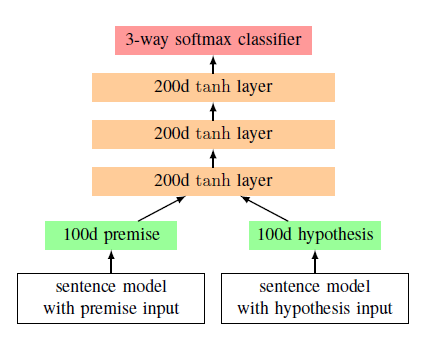
\includegraphics[width=0.6\linewidth]{pics/rnn-snli}
		\caption{Arsitektur RNN pada \textit{Textual Entailment} History \citep{snli:emnlp2015}}
		\label{fig:rnn-snli}
	\end{figure}
	Ada beberapa variasi percobaan yang \cite{snli:emnlp2015} lakukan, diantaranya arsitektur dikombinasikan dengan RNN biasa dan LSTM-RNN. Hasil percobaan menunjukkan \textit{Textual Entailment} dengan LSTM-RNN lebih unggul dibandingkan dengan RNN biasa, yaitu dengan perbandingan akurasi 77.6\% banding 72.2\%.
	
	Kemunculan SNLI memicu penelitian \textit{Textual Entailment} dengan menggunakan \textit{deep learning}, antara lain penelitian \cite{rnn-1}, \cite{rnn-2}, serta \cite{rnn-3}. Tujuan dari penelitian-penelitian tersebut adalah untuk menemukan variasi arsitektur RNN yang dapat meningkatkan akurasi dari penelitian \cite{snli:emnlp2015}. Ketiganya mengajukan bentuk arsitektur RNN yang berbeda-beda namun tetap mengujikannya dengan data SNLI. 
	
%-----------------------------------------------------------------------------%
\section{Evaluasi}
%-----------------------------------------------------------------------------%
Berdasarkan fungsinya, ada dua jenis evaluasi menurut Galliers dan Spark Jones \citep{Jones:1996:ENL:547445}, yaitu evaluasi intrinsik dan ekstrinsik. Evaluasi intrinsik dilakukan terkait tujuan sistem tersebut dibuat, sehingga evaluasi ini bisa dilakukan hanya dengan menilai hasil keluaran yang sistem itu sendiri.  Sedangkan evaluasi ekstrinsik dilakukan terhadap peranan dari sistem tersebut, sehingga butuh dilakukan \textit{task} lain untuk menguji hasil yang sistem keluarkan. Sebagai contoh, sebuah penelitian pengembangan korpus \textit{Textual Entailment} dapat dievaluasi menggunakan metode intrinsik dengan cara menilai akurasi dari hasil korpus yang terbentuk. Sedangkan, jika menggunakan pendekatan ekstrinsik, korpus tersebut bisa dinilai dengan cara mengaplikasikan korpus pada \textit{Textual Entailment} \textit{task}, seperti identifikasi hubungan \textit{entailment} pada \textit{testing data}.
	
Salah satu cara untuk menghitung suatu nilai evaluasi dari sebuah sistem klasifikasi adalah menggunakan akurasi. Akurasi adalah nilai pembagian dari data yang diklasifikasikan dengan benar terhadap jumlah seluruh data \citep{Manning:2008:IIR:1394399}. 
	\begin{equation}
	akurasi = \frac{jumlah\,\,data\,\,diklasifikasikan\,\,benar}{jumlah\,\,seluruh\,\,data}
	\end{equation}
	
	%-----------------------------------------------------------------------------%
	\subsection{Cross Validation}
	%-----------------------------------------------------------------------------%
	Evaluasi bisa dikombinasikan dengan teknik \textit{cross validation}. \textit{Cross validation} adalah sebuah teknik untuk memanfaatkan sejumlah data yang data tersedia dengan memecah data tersebut menjadi training dan testing data. Untuk mengurangi bias karena proses pemecahan data tersebut, dilakukan \textit{k-Fold cross validation}. \textit{K-fold cross validation} adalah salah satu jenis penggunaan \textit{cross validation} dengan pengulangan sebanyak \textit{k} kali \citep{olson2008advanced}. 
	\begin{figure}
		\centering
		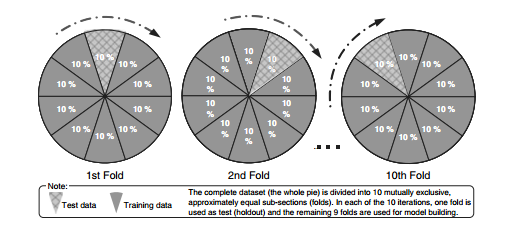
\includegraphics[width=0.7\linewidth]{pics/cv}
		\caption{Ilustrasi \textit{K-fold cross validation} \citep{olson2008advanced}}
		\label{fig:cv}
	\end{figure}
	\textit{Testing data} diambil sejumlah \textit{1/k} dari data total, data selebihnya menjadi \textit{training data}. Lalu pengujian dilakukan dan dihitung akurasinya. Hal tersebut diulangi hingga \textit{k} kali, yaitu ketika semua bagian data pernah menjadi \textit{testing data}. Akurasi keseluruhan adalah rata-rata akurasi pada tiap iterasi.
	
	
	
	%-----------------------------------------------------------------------------%
	\subsection{Kappa}
	%-----------------------------------------------------------------------------%
	Pada penelitian yang menggunakan anotator, evaluasi perlu dilakukan terhadap tingkat persetujuan antar anotator. Tingkat persetujuan tersebut dihitung menggunakan Kappa \citep{Manning:2008:IIR:1394399}. Berikut adalah persamaan umum suatu kappa.
	\begin{equation}
	Kappa = \frac{P(A)-P(E)}{1-P(E)}
	\end{equation}
	\noindent P(A) merupakan proporsi banyaknya nilai yang disetujui (\textit{agreement}) dan P(E) adalah proporsi banyaknya nilai yang disetujui karena ketidaksengajaan. 
	
	\cite{landis1977measurement} membagi rentang nilai Kappa menjadi beberapa tingkat persetujuan. Tabel \ref{table:skalaKappa} menunjukkan pembagian tersebut. 
	\begin{table}
		\centering
		\caption{Skala pengukuran Kappa \citep{landis1977measurement}}
		\label{table:skalaKappa}
		\begin{tabular}{|c|c|}
			\hline
			Statistik Kappa & Tingkat persetujuan \\ \hline
			<0.00 & \textit{poor} \\ \hline
			0.00 - 0.20 & \textit{slight} \\ \hline
			0.21 - 0.40 & \textit{fair} \\ \hline
			0.41 - 0.60 & \textit{moderate} \\ \hline
			0.61 - 0.80 & \textit{substantial} \\ \hline
			0.81 - 1.00 & \textit{almost perfect} \\ \hline
		\end{tabular}
	\end{table}
	\noindent Pengukuran Kappa pada tabel di atas kerap digunakan sebagai \textit{benchmark} dalam penelitian-penelitian yang menggunakan anotator.
	
	Kappa memiliki beberapa variasi perhitungan, antara lain Cohen's Kappa dan Fleiss Kappa. Cohen's Kappa digunakan untuk menghitung tingat persetujuan antar dua anotator \citep{Cohen1960}. Sedangkan, Fleiss Kappa \citep{fleiss1971measuring} bisa digunakan untuk menghitung tingkat persetujuan antara dua atau lebih anotator.
	Berikut adalah cara perhitungan \textit{P(A)} dan \textit{P(E)} pada Cohen's Kappa.
	\begin{table}
		\centering
		\caption{Perhitungan Cohen's Kappa}
		\label{table:cohenKappa}
		\begin{tabular}{|l|l|l|l|l|l|}
			\hline
			\multicolumn{2}{|l|}{\multirow{2}{*}{}} & \multicolumn{4}{c|}{\textbf{anotator 2}} \\ \cline{3-6} 
			\multicolumn{2}{|l|}{} & \textbf{label 1} & \textbf{label 2} & \textbf{...} & \textbf{label n} \\ \hline
			\multirow{4}{*}{\textbf{anotator 1}} & \textbf{label 1} & $m_{11}$ & $m_{12}$ & ... & $m_{1n}$ \\ \cline{2-6} 
			& \textbf{label 2} & $m_{21}$ & $m_{22}$ & ... & $m_{2n}$ \\ \cline{2-6} 
			& \textbf{...} & ... & ... & ... & ... \\ \cline{2-6} 
			& \textbf{label n} & $m_{n1}$ & $m_{n2}$ & ... & $m_{nn}$ \\ \hline
		\end{tabular}
	\end{table}
	\begin{equation}
	P(A) =\frac{\sum_{k=1}^{n} m_{kk}}{total\, data}
	\end{equation} 
	\begin{equation}
	P(E) =\frac{\sum_{k=1}^{n}(\sum_{j=1}^{n} m_{kj}\, \cdot \,\sum_{i=1}^{n} m_{ik})}{total\, data}
	\end{equation}
	\noindent dengan \textit{n} merupakan banyak label, dan $m_{ij}$ merupakan banyaknya data yang diberi label \textit{i} oleh anotator 1 dan label \textit{j} oleh anotator 2. Sedangkan, berikut adalah cara perhitungan \textit{P(A)} dan \textit{P(E)} pada Fleiss Kappa.
	\begin{equation}
	P(A) = \frac{1}{N}\sum_{i=1}^{N}P_{i}\:\:\:\:\:\:
	dengan\:\:\:\:\:\: P_{i} = \frac{1}{n(n-1)}[(\sum_{j=1}^{k}n_{ij}^{2})-(n)]
	\end{equation} 
	\begin{equation}
	P(E) = \sum_{i=1}^{k}P_{j}^{2}
	\end{equation}
	dengan \textit{N} merupakan jumlah data yang dianotasi, \textit{k} adalah jumlah label, \textit{n} adalah jumlah anotator, dan $n_{ij}$ adalah total anotator yang memberi label \textit{j} pada data ke-\textit{i}.